\documentclass{report}
\title{An Introductory Course in Computational Neuroscience---Paul Miller (Notes)}
\date{Started 14 Dec 2024}
\author{Malcolm}
\usepackage{amsmath} %import math
\usepackage{mathtools} %more math
\usepackage{amssymb} %for QED symbol
\usepackage{amsthm} %
\usepackage{bm} %bolding without changing font
\usepackage{graphicx} %import imaging
\graphicspath{{./images/}} %set imaging path
\newcommand*{\vertbar}{\rule[-1ex]{0.5pt}{2.5ex}} %matrix
\newcommand*{\horzbar}{\rule[.5ex]{2.5ex}{0.5pt}} %matrix
\begin{document}
\maketitle
\tableofcontents
\newpage

\section{xLIF}
\subsection{Modelling the Leaky membrane potential}
\textbf{Nernst Potential}\\
The \textit{Nernst potential} $E_A$ of an ion $A$ of charge $z_A$ with intracellular concentration $[A_{\text{in}}]$ and extracellular concentration $[A_{\text{out}}]$ is given by
\begin{equation*}
E_A=\frac{k_BT}{z_Aq_e}\ln\left(\frac{[A_{\text{out}}]}{[A_{\text{in}}]}\right)
\end{equation*}
where $T$ is the temperature in Kelvin, $k_B$ the Boltzmann constant $(1.39\times10^{-23}JK^{-1})$ (which converts units of temperature to units of thermal energy). $q_e$ is the fundamental electronic charge
$(1.60\times10^{-19}C)$.\\
\vspace{1mm}\\
\textbf{Model}\\
Considering this representation of a neuron's membrane:
\begin{figure}[h]
\begin{center}
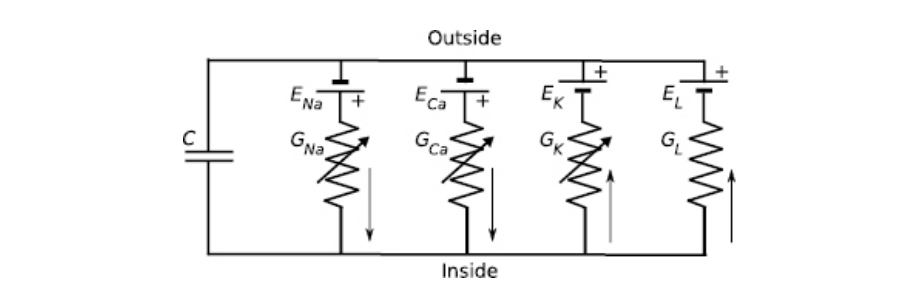
\includegraphics[width=10cm]{1}\\
\end{center}
If all channels with variable conductance are closed, then the current will only flow through the leak channels (subscript $L$) until the cell membrane is at the leak
potential $E_L$. The current through a channel is given by
\begin{equation*}
I_t=G_t(V_m-E_t)
\end{equation*}
Where $G_t$ represents conductance and $E_t$ the nernst potential; $t$ represents the type of channel.
\end{figure}\\
(next page)
\newpage
\noindent\textbf{Equilibrium}\\
When the cell is at equilibrium the different currents balance each other out and sum to zero:
\begin{equation*}
I_m=\sum_tI_t=\sum_tG_t(V_m-E_t)=0
\end{equation*}
In the context of this current model this can be rewritten as
\begin{equation*}
G_{Na}(V_m-E_{Na})+G_{Ca}(V_m-E_{Ca})+G_{K}(V_m-E_{K})
+G_{L}(V_m-E_{L})
\end{equation*}
Solving for $V_m$ we can see that the \textit{resting membrane potential}---where no net current flows, is the weighted average of the individual Nernst potentials:
\begin{equation*}
V_m=\frac{G_{Na}E_{Na}+G_{Ca}E_{Ca}+G_{K}E_{K}+G_{L}E_{L}}{G_{Na}+G_{Ca}+G_{K}+G_{L}}
\end{equation*}
The derivation of the resting membrane potential is typically more complicated.\\
\vspace{1mm}\\
\textbf{Leaky membrane potential}\\
Here we consider the passive properties of the cell, where the variable conductance of all channels are fixed. With this the we treat the circuit as having
a single `leak' conductance and potential.\\
\vspace{1mm}\\
The membrane potential is generated by the charge stored on the membrane; it depends on both the stored charge and the membrane's capacitance $C_m$ via the equation
\begin{equation*}
Q=C_mV_m
\end{equation*}
The current is defined as positive when it flows \textit{out} of the cell; with that we have
\begin{equation*}
\frac{dQ}{dt}=-I_m=-G_L(V_m-E_L)
\end{equation*}
Fixing the capacitance we obtain the dynamics of the resting membrane potential as
\begin{equation*}
C_m\frac{dV_m}{dt}=G_L(E_L-V_m)
\end{equation*}
This is a linear first order ODE. 
\newpage

\subsection{Solution for Leaky ODE}
We had the dynamics of the resting membrane potential as
\begin{equation*}
C_m\frac{dV_m}{dt}=G_L(E_L-V_m)
\end{equation*}
Expressing in standard form and solving by integrating factor:
\begin{align*}
\frac{dV_m}{dt}+\frac{G_L}{C_m}V_m&=\frac{G_L}{C_m}E_L\\
V_m&=\frac{1}{\exp\left(\frac{G_L}{C_m}t\right)}\left(\int\exp\left(\frac{G_L}{C_m}t\right)\cdot\frac{G_L}{C_m}E_L\,dt+c\right)
\end{align*}
To simplify we define the \textit{time constant} $\tau_m=C_m/G_L$:
\begin{align*}
V_m&=\frac{1}{\exp\left(\frac{t}{\tau_m}\right)}\left(\int\exp\left(\frac{1}{\tau_m}t\right)\cdot\frac{1}{\tau_m}E_L\,dt+c\right)\\
&=\exp\left(-\frac{t}{\tau_m}\right)\left(\exp\left(\frac{t}{\tau_m}\right)E_L+A\right)\\
&=E_L+\exp\left(-\frac{t}{\tau_m}\right)\cdot A
\end{align*}
At initial condition $V_m(0)$:
\begin{equation*}
V_m(0)=E_L+A\implies A=V_m(0)-E_L
\end{equation*}
With that we have the solution
\begin{equation*}
V_m=E_L+(V_m(0)-E_L)\exp\left(-\frac{t}{\tau_m}\right)
\end{equation*}
(next page)
\newpage
\noindent\textbf{Illustrated}\\
See that the equation tends to $E_L$, and that $\tau_m$ dictates how fast this decay occurs (thus the name). Illustrated here using code from \texttt{leakymembrane.py}:
\begin{figure}[h]
\begin{equation*}
V_m=E_L+(V_m(0)-E_L)\exp\left(-\frac{t}{\tau_m}\right)
\end{equation*}
\begin{center}
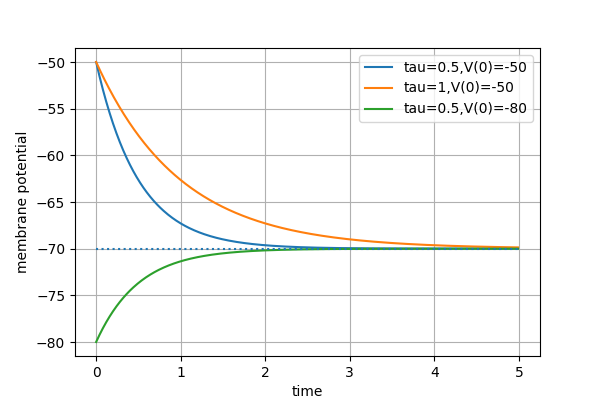
\includegraphics[width=10cm]{2}\\
\end{center}
\end{figure}















\end{document}
